\section{Self-Improving Frontier Discovery}
\label{sec:frontier}

A defining feature of WuYa is its ability to learn from interactions and improve its evaluation capabilities over time. Inspired by Reflexion's verbal reinforcement learning and Voyager's skill library, we introduce a frontier discovery mechanism that captures and accumulates evaluation preferences.

\subsection{Motivation: The Static Knowledge Problem}

Existing academic evaluation systems deploy fixed criteria that do not adapt to:
\begin{itemize}
    \item Evolving disciplinary standards (e.g., increasing emphasis on reproducibility).
    \item Journal-specific preferences (e.g., some journals prioritize theory, others prioritize application).
    \item Feedback from editors and reviewers.
\end{itemize}

This static knowledge problem is particularly acute for \dea{} analysis, which depends on reference frontiers that may become outdated as a field evolves.

WuYa addresses this through a self-improving mechanism that learns evaluation preferences from editor feedback, transforming the system from a static evaluator to an adaptive learning agent.

\subsection{Comparison with Existing Frameworks}

WuYa's frontier discovery draws inspiration from two influential self-improving agent frameworks:

\textbf{Reflexion \citep{shinn2023reflexion}} introduced verbal reinforcement learning where agents store linguistic reflections in episodic memory and use them to guide future decisions. When a task fails, the agent generates a verbal reflection explaining \textit{why} it failed and stores this in memory for future reference. This has proven effective for code generation and game playing tasks.

\textbf{Voyager \citep{wang2023voyager}} proposed an open-ended agent that builds a skill library through embodied exploration. Skills are represented as executable code snippets that enable the agent to solve progressively complex tasks. The library grows over time, enabling lifelong learning.

WuYa adapts these principles to academic evaluation:

\begin{itemize}
    \item Like Reflexion, WuYa generates \textbf{linguistic reflections} on evaluation outcomes, but from editor/reviewer feedback rather than task success/failure.
    \item Like Voyager, WuYa maintains a \textbf{library of learned patterns}, but these are ``frontier surfaces'' capturing evaluation preferences rather than executable skills.
\end{itemize}

Table~\ref{tab:frontier-comparison} summarizes the comparison.

\begin{table}[t]
\centering
\caption{WuYa Frontier Discovery vs. Existing Frameworks}
\label{tab:frontier-comparison}
\begin{tabular}{@{}llll@{}}
\toprule
\textbf{Aspect} & \textbf{Reflexion} & \textbf{Voyager} & \textbf{WuYa Frontier Discovery} \\
\midrule
Learning Signal & Task success/failure & Environment feedback & Editor/reviewer feedback \\
Memory Form & Episodic reflections & Skill library (code) & Frontier surfaces (preferences) \\
Update Trigger & Task completion & Skill discovery & Review cycle completion \\
Retrieval Coupling & None & Skill retrieval & Canonical text retrieval \\
Domain & Verifiable & Embodied & Evaluative \\
\bottomrule
\end{tabular}
\end{table}

\subsection{Frontier Discovery Sub-agent}

The Frontier Discovery \subagent{} operates as a background process that continuously learns from interactions. Its workflow consists of three stages:

\begin{enumerate}
    \item \textbf{Feedback Reception}: Receives structured input from completed review cycles:
    \begin{itemize}
        \item Paper's five-dimensional score vector.
        \item Editor/reviewer feedback text.
        \item Journal acceptance/rejection decision.
        \item Post-review correspondence (rebuttal, revision).
    \end{itemize}
    \item \textbf{Linguistic Reflection}: Generates structured descriptions of evaluation patterns:
    \begin{verbatim}
    {
      "journal_id": "Nature ML",
      "pattern": {
        "dimension": "innovation",
        "preference": "prefers paradigm shifts over incremental improvements",
        "evidence": [
          "Reviewer 1: 'lacks the conceptual breakthrough...'", 
          "Decision: '...findings are incremental...'"
        ],
        "confidence": 0.82
      }
    }
    \end{verbatim}
    \item \textbf{Frontier Surface Update}: Incorporates new patterns into the frontier surface library:
    \begin{verbatim}
    {
      "journal_id": "Nature ML",
      "frontier_surface": {
        "description": "Innovation frontier emphasizes 
                         paradigm shifts and knowledge bridging",
        "score_distribution": {"Q1-A": 0.3, "Q1-B": 0.4, ...},
        "updated_at": "2026-05-26",
        "patterns": [...]
      }
    }
    \end{verbatim}
\end{enumerate}

\subsection{Frontier Surface Library}

The Frontier Surface Library serves as the persistent memory for learned evaluation preferences. It is organized hierarchically:

\begin{itemize}
    \item \textbf{Journal Level}: Individual frontier surfaces for each journal, capturing that journal's specific evaluation preferences.
    \item \textbf{Discipline Level}: Aggregated frontier surfaces for each academic discipline.
    \item \textbf{Global Level}: Cross-cutting patterns that transcend disciplines.
\end{itemize}

The library is queried during paper localization to:
\begin{itemize}
    \item Customize recommendations based on journal-specific preferences.
    \item Weight evaluation dimensions differently for different journals.
    \item Update \dea{} reference frontiers with learned patterns.
\end{itemize}

\subsection{Self-Improvement Loop}

WuYa implements a continuous self-improvement loop:

\begin{figure}[t]
    \centering
    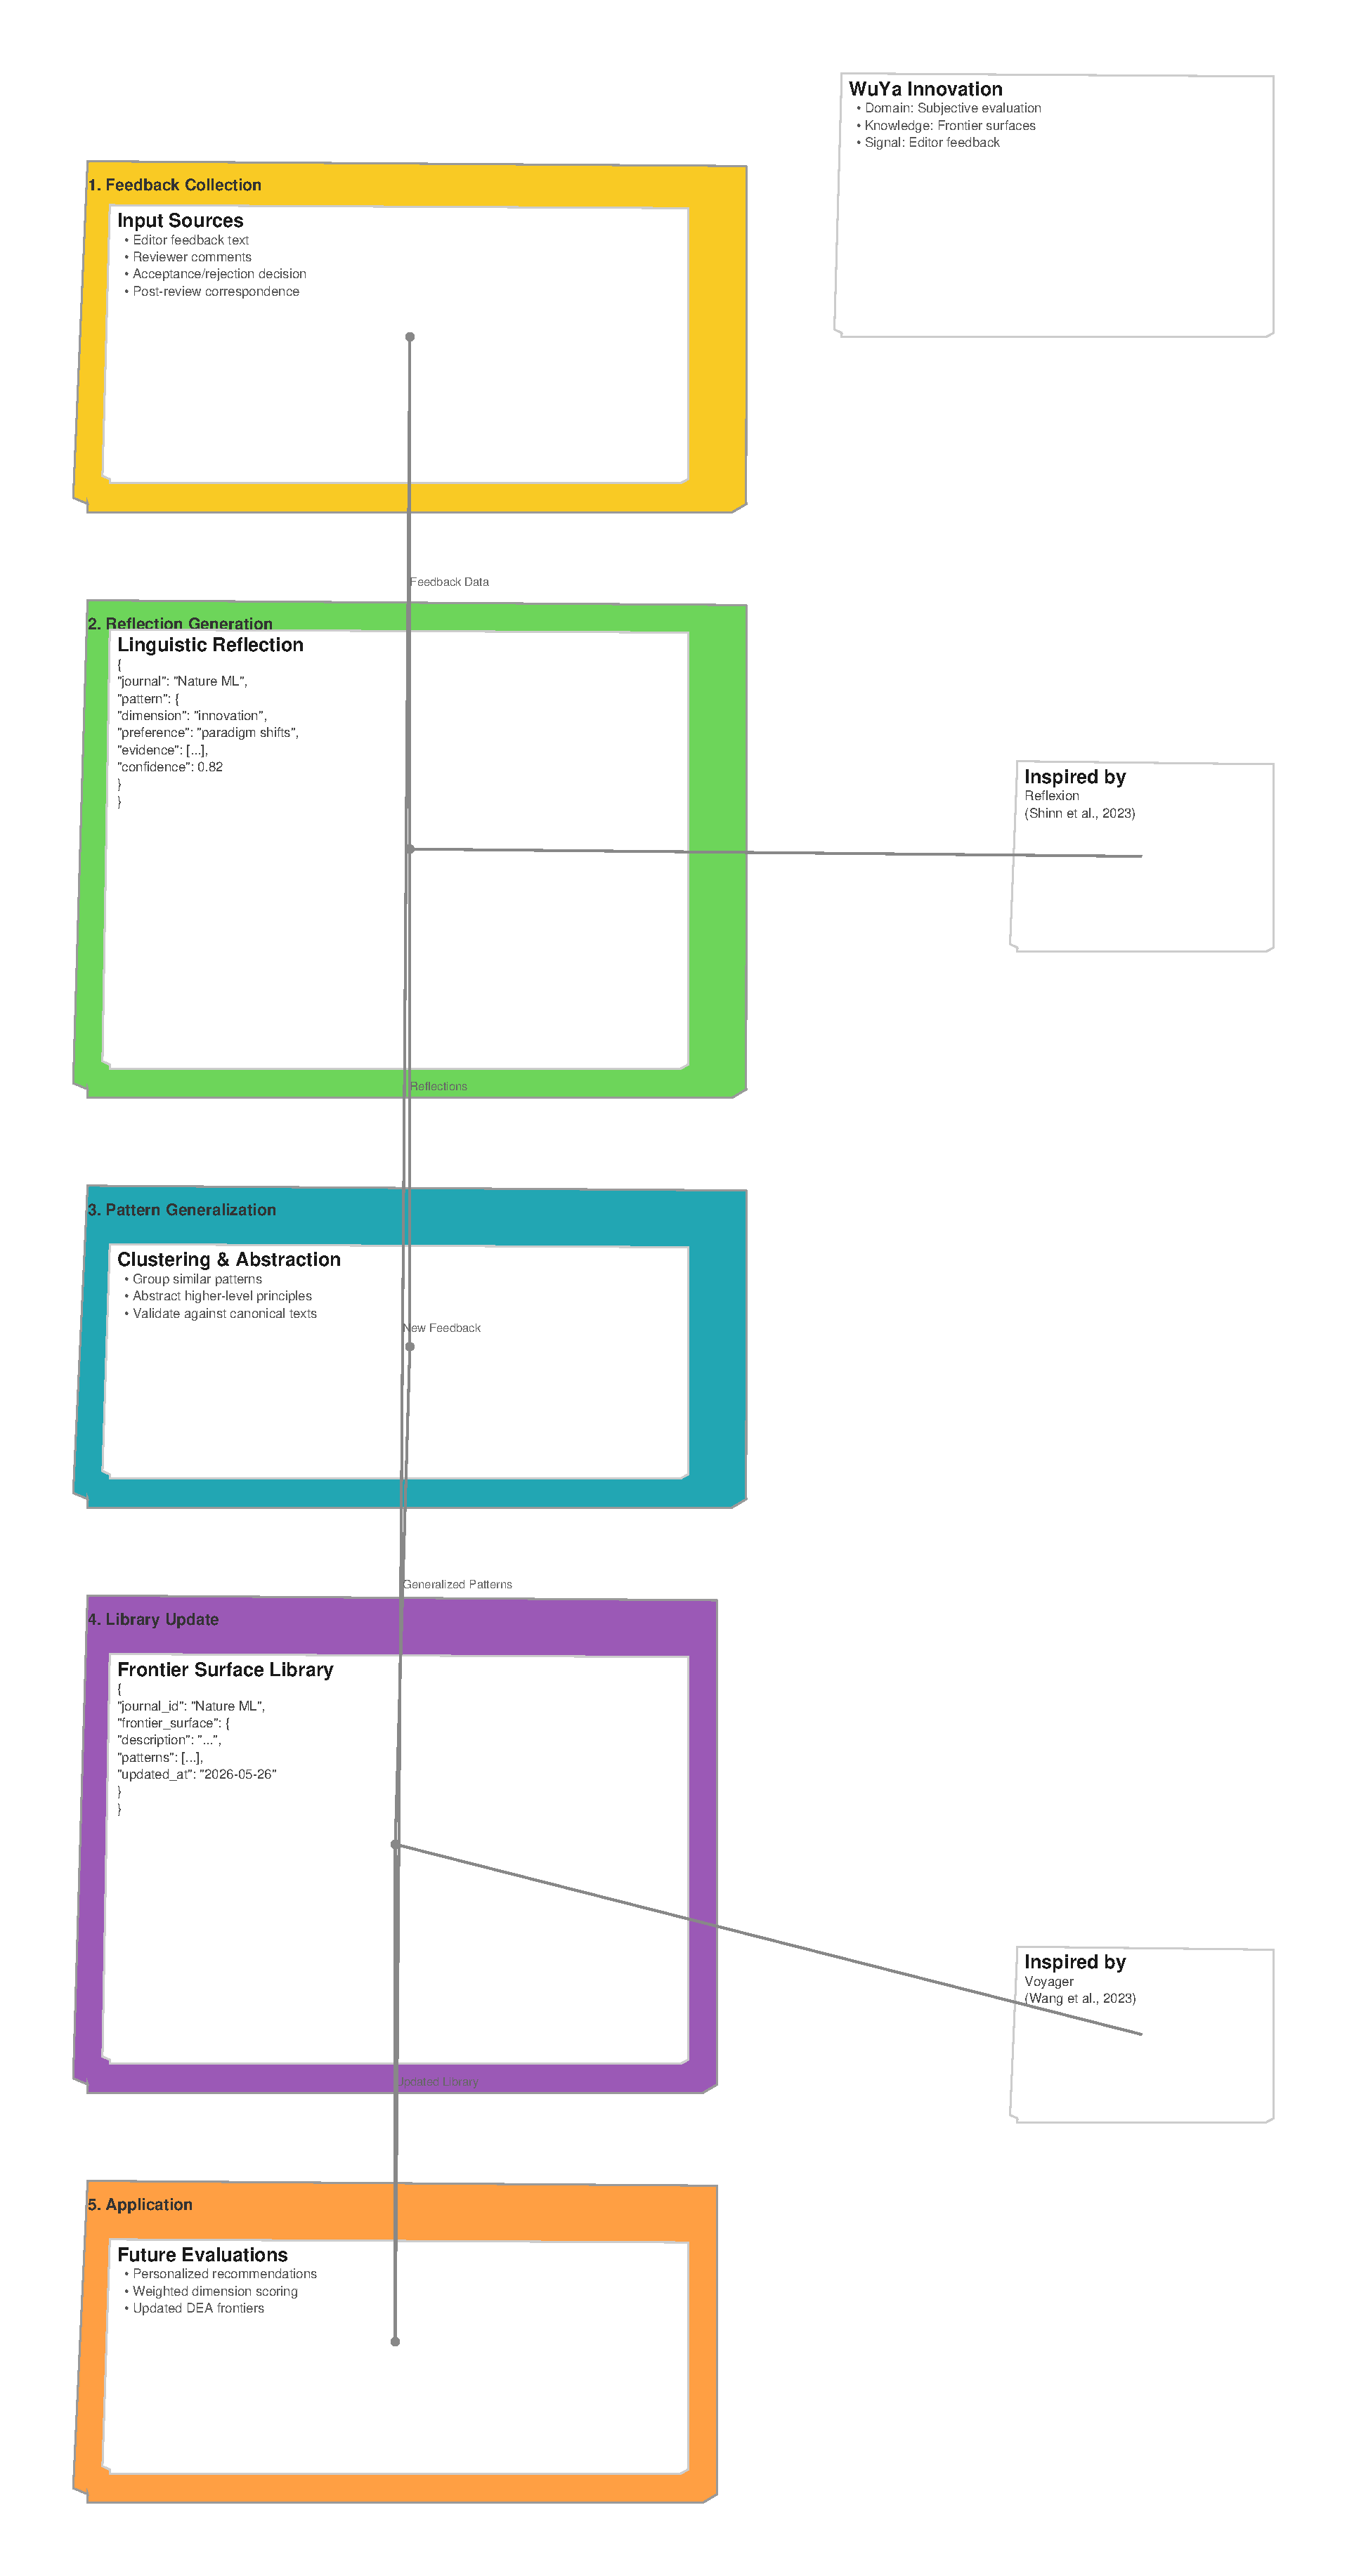
\includegraphics[width=0.8\textwidth]{figures/self-improvement-loop.pdf}
    \caption{WuYa Self-Improvement Loop: Feedback $\rightarrow$ Reflection $\rightarrow$ Generalization $\rightarrow$ Application}
    \label{fig:self-improvement}
\end{figure}

\begin{enumerate}
    \item \textbf{Feedback Collection}: Editor/reviewer feedback is collected during and after review cycles.
    \item \textbf{Reflection Generation}: The Frontier Discovery \subagent{} generates linguistic reflections on evaluation patterns.
    \item \textbf{Pattern Generalization}: Related patterns are clustered and abstracted to form higher-level principles.
    \item \textbf{Library Update}: New patterns are incorporated into the Frontier Surface Library.
    \item \textbf{Application}: Updated knowledge informs future evaluations, recommendations, and \dea{} frontiers.
\end{enumerate}

This loop enables WuYa to:
\begin{itemize}
    \item Adapt to changing disciplinary standards over time.
    \item Capture journal-specific evaluation preferences without manual configuration.
    \item Improve \dea{} frontier quality through accumulated learning.
    \item Provide increasingly personalized recommendations as the system matures.
\end{itemize}

\subsection{Contrast with Static Knowledge Bases}

Traditional academic evaluation systems use static knowledge bases that:
\begin{itemize}
    \item Require manual curation and updates.
    \item Do not capture subtle journal-specific preferences.
    \item Cannot adapt to evolving disciplinary standards.
    \item Depend entirely on predefined criteria.
\end{itemize}

WuYa's Frontier Surface Library overcomes these limitations through:
\begin{itemize}
    \item \textbf{Automatic learning}: Patterns emerge from actual editor feedback rather than expert curation.
    \item \textbf{Granular capture}: Individual journal preferences are preserved in separate frontier surfaces.
    \item \textbf{Dynamic adaptation}: The library evolves as the field advances.
    \item \textbf{ Principled grounding}: Learned patterns are validated against canonical texts through \rag{}.
\end{itemize}
